% !TeX program = xelatex
% VulnHunter 中文预印本框架稿。由 Henriques Lab bioRxiv 样式改写。
% 本稿中的 nan 是待实验占位值，不代表任何已测结果。
\documentclass[times,twoside,watermark]{zHenriquesLab-StyleBioRxiv}
\usepackage{xeCJK}
\setCJKmainfont{FandolSong-Regular}
\setCJKsansfont{FandolHei-Regular}
\usepackage{booktabs,tabularx,array,float}
\usepackage{microtype}
\usepackage{balance}
\widowpenalty=10000
\clubpenalty=10000
\displaywidowpenalty=10000
\newcommand{\VH}{\textsc{VulnHunter}}
\newcommand{\nan}{\texttt{nan}}
\newcommand{\PC}{\operatorname{PC}}
\leadauthor{VulnHunter}

\begin{document}
\title{VulnHunter：融合程序分析与动态验证的\\仓库级漏洞审计框架}
\shorttitle{VulnHunter 中文预印本草稿}
\author[1]{作者待补充}
\affil[1]{单位待补充}
\maketitle

\begin{abstract}
仓库级漏洞检测需要结合目标函数、跨文件调用关系及实际运行条件，仅凭局部代码片段或单一静态告警难以判断安全影响是否成立。本文介绍 \VH{}，一个面向 Python 仓库的代理式漏洞审计框架。主审计代理按需阅读仓库上下文，并调用 CodeQL、Semgrep 与基于代码属性图的 CodeBadger 形成待验证的漏洞假设；独立执行代理在任务专属容器中尝试复现，将过程中的事实与证据引用追加到黑板，再由主代理生成结构化判定和报告。本文给出任务输入、证据流转、动态验证和结果契约的实现设计，并规划以 DREA 为主基线，在相同的 RepoPairBench 100 样例上比较检测能力、报告可核查性及运行成本。当前文稿为实验前框架稿，\VH{} 的性能与成本结果均以 \nan{} 占位，不据此主张系统优于任何基线。
\end{abstract}

\begin{keywords}
关键词：仓库级漏洞检测；大语言模型代理；程序分析；动态验证；证据可追溯
\end{keywords}

\section*{引言}
软件漏洞的触发条件往往分散在多个函数和文件中。目标函数中的危险操作可能受到调用方权限检查保护，也可能只在特定配置、依赖版本或输入形态下被触发。基于固定代码片段作判断容易遗漏这些条件；把静态工具产生的候选路径直接等同于可利用漏洞，也可能导致误报。已有研究将目标导向的仓库探索用于漏洞检测，并提出按修复前后版本配对的评估方式\cite{drea2026}。

本文关注从\emph{可疑线索}走向\emph{可核查结论}的过程。代码阅读和程序分析有助于形成漏洞假设，执行环境则可以观察部分假设对应的运行时行为，但动态验证会受到依赖安装、入口构造与运行预算的限制。因此，审计系统需要记录证据来源、区分观察与推断，并明确说明无法复现时的判定语义。

\VH{} 将上述过程组织为两个职责分离的代理：主审计代理负责仓库探索和假设更新，执行代理通过 Docker 工具在任务容器中尝试验证。系统以追加事件形式维护事实黑板，并要求最终输出结构化结论。本文的研究问题为：（1）多源程序分析如何支持目标函数的漏洞假设构造；（2）动态观察和事件式记录能否提高报告的可复核性；（3）严格的阳性确认门槛对召回率、误报率和无法判定样例有何影响。第三个问题必须通过后续实验回答，本文不预设结果。

本文贡献以可核实的系统设计和可复现的评测协议为主：给出目标函数与仓库快照的联合输入流程；描述主审计代理、容器执行代理及事件黑板之间的证据传递；定义同时报告单样例检测、修复对正确性、运行覆盖与证据质量的实验方案。

\section*{任务定义与系统概览}
对一个漏洞修复对，记修复前仓库为 $R_i^{-}$，修复后仓库为 $R_i^{+}$，对应目标函数为 $f_i^{-}$ 与 $f_i^{+}$。系统输入为 $(R_i^s,f_i^s)$，其中 $s\in\{-,+\}$；期望标签为 $y_i^{-}=1$、$y_i^{+}=0$。审计输出二值标签 $\hat y_i^s$，并在阳性时附带漏洞位置、触发条件、复现步骤、观察结果及证据引用。任务范围限定为给定目标函数，避免把仓库中其他缺陷计作本样例的正确发现。

本文将\emph{线索}定义为代码或工具返回的可疑操作，将\emph{假设}定义为关于攻击者控制、传播路径和安全影响的解释，将\emph{观察}定义为在执行环境中实际记录的行为。线索和假设不能自动替代观察。图~\ref{fig:flow} 展示当前实现的审计数据流。

\begin{figure*}[t]
\centering
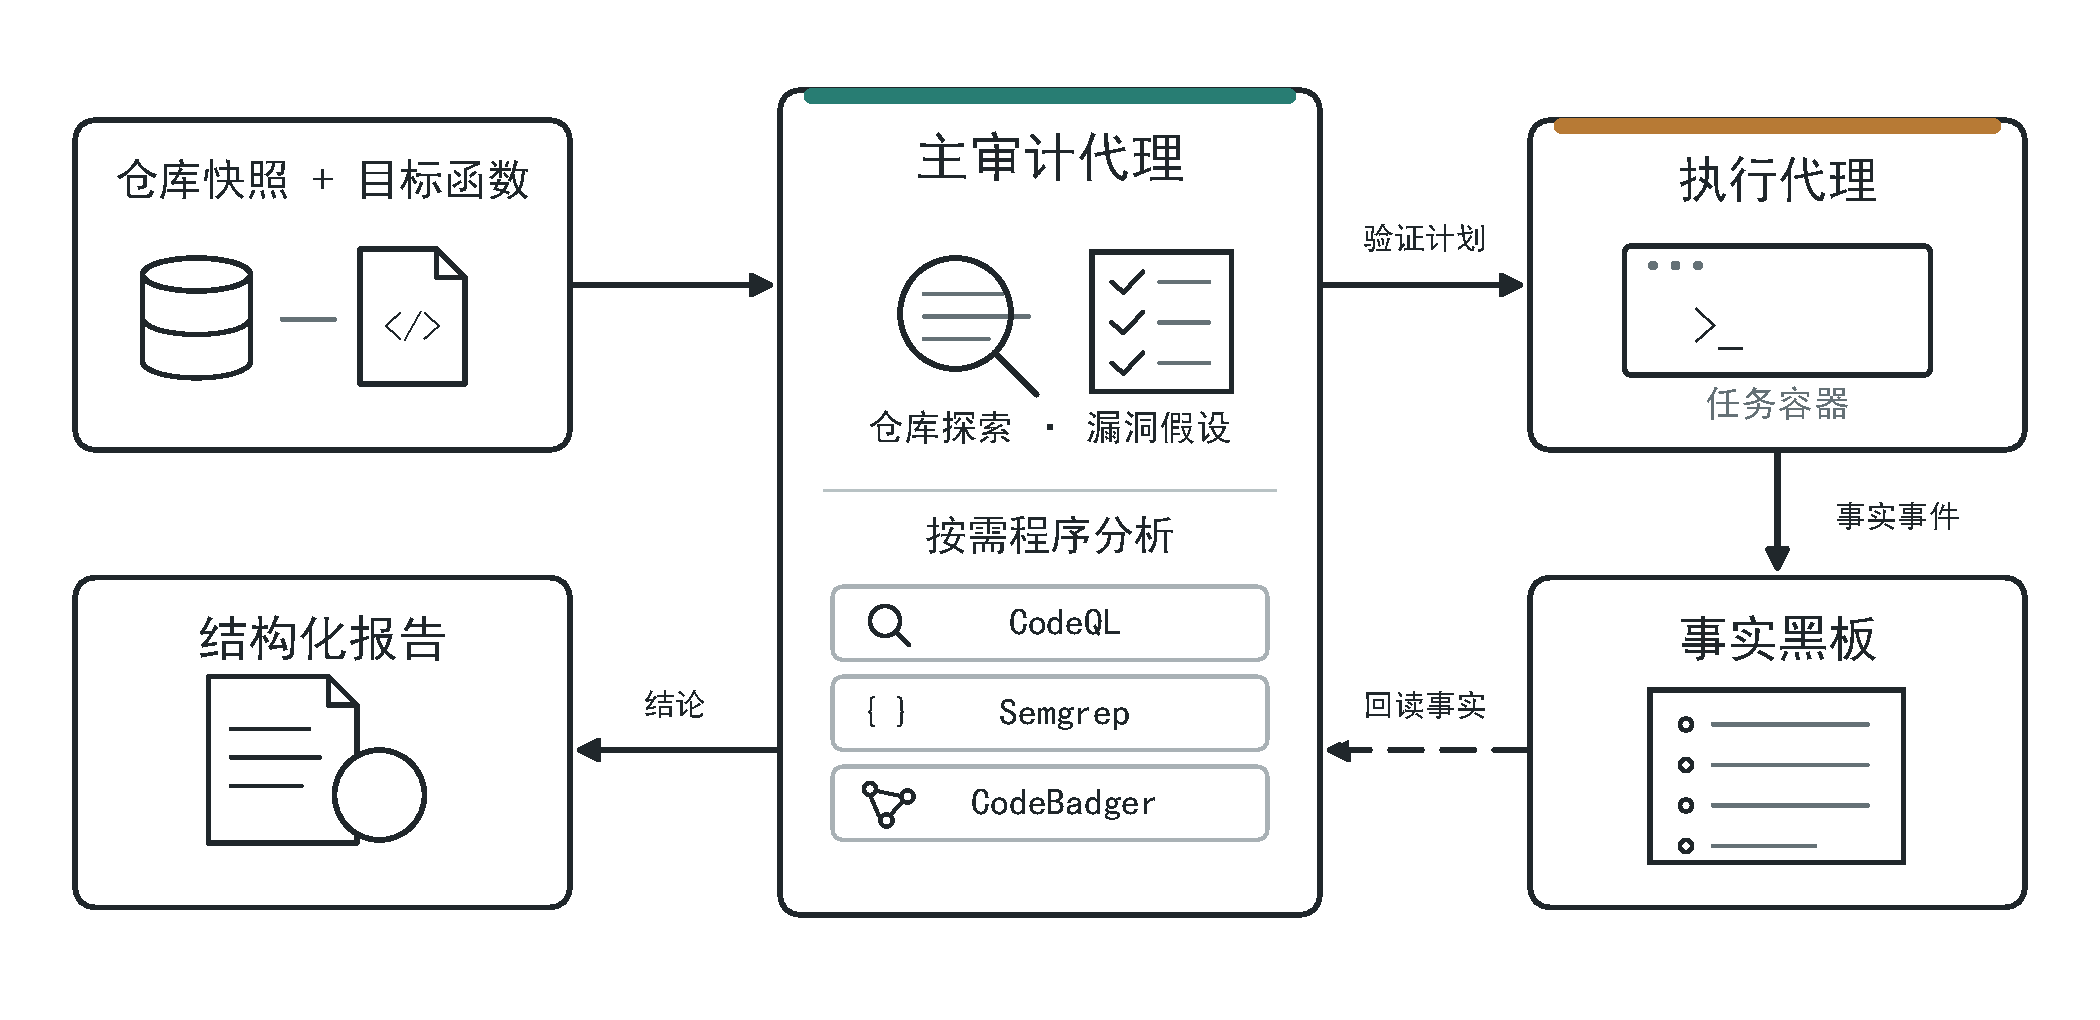
\includegraphics[width=0.95\textwidth]{Figures/VulnHunter-figure1-studio-pro.pdf}
\caption{\VH{} 的审计数据流。主代理按需查询程序分析工具并制定验证计划；执行代理在任务容器中尝试验证，将事实事件追加到黑板。虚线表示主代理回读事件。}
\label{fig:flow}
\end{figure*}

\section*{方法}
\subsection*{目标导向的仓库探索}
主代理读取目标文件，并根据当前假设扩展到调用方、被调用函数、配置和相关测试。CodeQL、Semgrep 与 CodeBadger 分别提供不同形式的程序分析接口。CodeBadger 使用基于 Joern 的代码属性图查询；代码属性图将程序的不同结构统一表示，适合表达跨语法和数据流关系\cite{cpg2014}。这些工具用于产生或核查线索，系统没有固定要求每个任务调用全部工具，也没有将告警数量直接映射为最终标签。

\subsection*{隔离式动态验证}
当主代理形成可执行的漏洞假设后，执行代理收到与当前目标相关的验证计划。该代理配置了 Docker MCP 工具与黑板追加工具，在任务专属容器的工作目录中检查依赖、构造输入并尝试触发安全影响。动态状态区分已确认、未确认与无法判断；仅有静态可疑路径、理论性 PoC 或运行失败，均不能作为已观察到的攻击成功。容器为任务提供执行环境与资源归属，但本文不把它描述为完全封闭的安全沙箱。任务结束时的清理流程释放相关分析作业，并停止、移除任务容器。

\subsection*{事件式事实黑板}
执行代理以包含事件标识、事实列表和可选证据引用的记录向黑板追加信息。合并过程按事件标识去重，并拒绝同一标识对应不同内容的静默覆盖；主代理随后从事件集合重建可读上下文。该设计针对并发及重试中的记录丢失问题，保证的是事件合并规则，而不是事实的真实性。黑板允许没有证据引用的事件，因此后续实验还需单独检查报告证据与原始工具输出是否一致。

\subsection*{结构化结论}
当前结果模式只输出二值判定：阳性包含漏洞报告，阴性不含阳性报告。提示要求观察到攻击影响后才判阳性；模式校验只验证字段关系，不核验动态证据。环境失败或无法复现可能被压为阴性，正式实验需单独报告这些状态。

\section*{实验设计}
\subsection*{数据与运行协议}
主评测拟使用仓库已导入的 RepoPairBench 100。该集合包含 100 组 Python 漏洞修复对，双侧运行对应 200 个实例；这些是数据集定义和本地元数据规模，并非模型实验结果。对每一对，漏洞侧检出修复提交的父版本，修复侧检出修复提交；两侧分别提供仓库快照、目标文件路径和函数代码。评测输入不直接提供 CVE 或 CWE 标签。所有运行需要固定代码提交、模型及推理参数、工具版本、容器镜像、预算和并发设置，并保存逐样例状态与轨迹。



\subsection*{指标与分母}
记漏洞侧正确判阳性为 TP、判阴性为 FN，修复侧误判阳性为 FP、正确判阴性为 TN。主要指标定义为
\begin{align}
\mathrm{Recall}&=\frac{\mathrm{TP}}{\mathrm{TP}+\mathrm{FN}},&
\mathrm{FPR}&=\frac{\mathrm{FP}}{\mathrm{FP}+\mathrm{TN}},\\
\mathrm{Precision}&=\frac{\mathrm{TP}}{\mathrm{TP}+\mathrm{FP}},&
F_1&=\frac{2\mathrm{TP}}{2\mathrm{TP}+\mathrm{FP}+\mathrm{FN}}.
\end{align}
修复对正确性要求同一对的漏洞版判阳性、修复版判阴性：
\begin{equation}
\PC=\frac{\sum_i\mathbf{1}[\hat y_i^{-}=1\land\hat y_i^{+}=0]}
{N_{\mathrm{complete\ pairs}}}.
\end{equation}
实验还应报告准确率、Youden $J=\mathrm{Recall}-\mathrm{FPR}$、有效覆盖数，以及失败、取消和无法解析判定的数量。未执行完成的样例不进入二值混淆矩阵；已执行但没有有效判定的样例应在相应标签侧按漏判或误报处理，并单列状态。只有两侧都有有效判定的修复对才进入 $\PC$ 的分母，须同时公布这个分母。

\begin{table}[H]
\centering
\caption{主实验结果占位表。所有性能与运行数据待测。}
\label{tab:main}
\begin{tabular}{lr}
\toprule
指标 & \VH{}\\
\midrule
完成实例 / 计划实例 & \nan{} / \nan{}\\
TP / FN / FP / TN & \nan{} / \nan{} / \nan{} / \nan{}\\
Recall / FPR & \nan{} / \nan{}\\
Precision / $F_1$ / Accuracy & \nan{} / \nan{} / \nan{}\\
成对正确 / 完整对数 & \nan{} / \nan{}\\
无法解析 / 失败 / 取消 & \nan{} / \nan{} / \nan{}\\
\bottomrule
\end{tabular}
\end{table}

\subsection*{与 DREA 的主基线对比}
DREA 是本文的主对照系统。其论文在 RepoPairBench 的 100 个修复对上报告 Recall、FPR、$F_1$、成对正确率与 Youden $J$，并分别使用 DeepSeek-V3.2、GLM-4.7 和 GPT-5.2 作为主模型\cite{drea2026}。表~\ref{tab:drea} 录入论文表 1 的 DREA 原值，为后续填入 \VH{} 的同模型结果预留位置；这些文献值不是本文复现实验。

\begin{table}[H]
\centering\footnotesize
\caption{DREA 检测指标对照。每格为 DREA 文献原值 / \VH{} 待测值；除 $J$ 为百分点外，单位均为百分比。}
\label{tab:drea}
\begin{tabular}{lccc}
\toprule
指标 & DeepSeek-V3.2 & GLM-4.7 & GPT-5.2\\
\midrule
Recall & 80.0/\nan{} & 59.0/\nan{} & 53.0/\nan{}\\
FPR & 45.0/\nan{} & 38.0/\nan{} & 28.0/\nan{}\\
$F_1$ & 71.1/\nan{} & 59.9/\nan{} & 58.6/\nan{}\\
P-C & 42.0/\nan{} & 34.0/\nan{} & 30.0/\nan{}\\
$J$ & 35.0/\nan{} & 21.0/\nan{} & 25.0/\nan{}\\
\bottomrule
\end{tabular}
\end{table}

为避免单个指标掩盖成对错误，表~\ref{tab:pair} 沿用 DREA 的四类结果：P-C 为双侧正确，P-V 为双侧判阳性，P-B 为双侧判阴性，P-R 为标签颠倒。DREA 的每个模型覆盖全部 100 对；\VH{} 应同时报告有完整有效判定的对数，不得在覆盖不足时直接比较计数。

\begin{table}[H]
\centering\footnotesize
\caption{修复对结果分解。每格为 DREA 文献计数 / \VH{} 待测计数。}
\label{tab:pair}
\begin{tabular}{lccc}
\toprule
类别 & DeepSeek-V3.2 & GLM-4.7 & GPT-5.2\\
\midrule
P-C & 42/\nan{} & 34/\nan{} & 30/\nan{}\\
P-V & 38/\nan{} & 25/\nan{} & 23/\nan{}\\
P-B & 13/\nan{} & 28/\nan{} & 42/\nan{}\\
P-R & 7/\nan{} & 13/\nan{} & 5/\nan{}\\
\bottomrule
\end{tabular}
\end{table}

运行成本按每个有效样例分别统计总 Token、付费 API Token 与本地模型 Token。表~\ref{tab:tokens} 给出 DREA 论文表 4 的原值；其成本节省倍数基于假设性计费方式，不能视为包含本地 GPU 的总费用。\VH{} 还需另报容器执行与分析工具的耗时和资源使用。

\begin{table}[H]
\centering\footnotesize
\caption{平均每样例 Token 用量，单位为千 Token；DREA 文献值四舍五入至一位小数，每格为 DREA / \VH{}。}
\label{tab:tokens}
\begin{tabular}{lccc}
\toprule
类型 & DeepSeek-V3.2 & GLM-4.7 & GPT-5.2\\
\midrule
总量 & 1397.7/\nan{} & 1560.5/\nan{} & 345.7/\nan{}\\
API & 87.8/\nan{} & 32.6/\nan{} & 8.4/\nan{}\\
本地 & 1309.8/\nan{} & 1528.0/\nan{} & 337.3/\nan{}\\
\bottomrule
\end{tabular}
\end{table}
正式比较须使用相同的目标函数与修复前后仓库快照、相同主模型版本、明确的解码参数与推理预算，并报告失败和无效输出的处理方式。若无法使用论文中的主模型，表~\ref{tab:drea} 只能作为外部参考；应另行复现 DREA，不能把不同模型下的分数差异归因于审计框架。DREA 的推理正确率仅在真正例上由裁判模型核验，若本文报告该指标，也必须使用相同标签资料、评价准则和分母。Token 与费用比较需区分付费 API 调用和本地执行资源，不能把 DREA 的估算节省倍数当作实测总费用。
\subsection*{内部消融与案例}
外部性能基线仅为 DREA。为分析 \VH{} 内部模块的作用，拟在相同目标函数、仓库快照、主模型与预算下，分别关闭 CodeQL、Semgrep 或 CodeBadger；这些配置只用于内部消融，不作为其他系统的对照。表~\ref{tab:ablation} 预留结果位置，实验组尚需实现和运行。
\begin{table}[H]
\centering
\caption{计划中的消融实验；表中结果均未产生。}
\label{tab:ablation}
\begin{tabular}{lccc}
\toprule
配置 & Recall & FPR & $\PC$\\
\midrule
完整 \VH{} & \nan{} & \nan{} & \nan{}\\
移除 CodeQL & \nan{} & \nan{} & \nan{}\\
移除 Semgrep & \nan{} & \nan{} & \nan{}\\
移除 CodeBadger & \nan{} & \nan{} & \nan{}\\
\bottomrule
\end{tabular}
\end{table}

除检测标签外，实验还应测量每例调用次数、输入输出 Token、运行时间和动态验证状态，并抽样核对阳性报告中的证据引用。案例分析至少覆盖正确定位、修复版误报、漏洞版漏报和环境失败四类轨迹。对每类案例，应按“线索—假设—执行观察—最终结论”的顺序复盘，避免只展示结论正确的成功案例。

\balance
\section*{结果分析框架}
表~\ref{tab:main} 至表~\ref{tab:tokens} 目前给出 DREA 文献值与 \VH{} 的待测口径，不支持任何关于性能提升的结论。获得正式结果后，将先核对完成量与分母，再比较漏洞侧召回和修复侧误报，最后检查\mbox{成对正确性}。若单样例准确率与成对正确率出现差异，应进一步按“双侧均阳性”“双侧均阴性”“标签颠倒”等错误形态拆解。对消融结果的解释还需结合工具调用轨迹：某工具未被使用的样例，不能用来支持其对该样例判定产生了影响的主张。

动态证据分析将分别统计已确认、未确认、环境失败和未执行数量，并检查“有证据引用”与“证据足以支持结论”之间的差别。时间、Token 与容器资源消耗应与检测质量共同报告，不应仅用准确率评价代理的实用性。

\section*{效度威胁与局限}
\paragraph{严格阳性门槛。} 环境依赖缺失或入口无法构造时，未观察到攻击效果不等于漏洞不存在。当前二值输出可能将无法判断压成阴性。正式评测应公布环境失败率与有效覆盖率，并在讨论中区分保守判定造成的漏报和真实无漏洞样例。

\paragraph{证据真实性。} 事件黑板能够防止已记录事件被旧状态覆盖，却不会自动检查代理描述是否准确。最终报告中的复现命令、工具输出与观察现象需要通过保存的原始轨迹复核。

\paragraph{可比性与泛化。} 公开修复提交可能通过仓库历史泄露标签线索；评测应审查工具调用是否读取了补丁或提交信息。RepoPairBench 100 主要覆盖 Python 公开修复对，结果不能直接推广到其他语言或未公开漏洞。不同代理若使用不同模型、预算或判定门槛，也不能把分数差异归因于系统架构。

\section*{相关工作}
ReAct 将推理与环境动作交替组织，为可调用工具的语言模型代理提供了通用交互模式\cite{react2023}。SWE-agent 研究面向软件工程任务的代理计算机接口及仓库操作方式\cite{sweagent2024}。DREA 将仓库级漏洞检测中的推理与探索分工，并提供修复前后配对的 RepoPairBench\cite{drea2026}。\VH{} 与这些工作共享代理式仓库探索的背景，本文聚焦的是静态线索、动态观察和报告证据在单次审计中的连接。代码属性图研究为跨结构的漏洞分析提供了程序表示基础\cite{cpg2014}。

\section*{结论}
本文给出 \VH{} 中文预印本的系统与实验框架：主代理按需获取程序分析线索，执行代理在任务容器中尝试验证，事实黑板保存事件，最终输出结构化报告。检测效果、证据质量及资源开销尚待在固定配置的配对实验中测量，文中所有 \nan{} 均需用可追溯的实测数据替换。后续定稿还需补齐作者信息、正式对照结果、代表性案例和复现实验材料。

\section*{参考文献}
\bibliography{references}
\end{document}














